\iffalse
\let\negmedspace\undefined
\let\negthickspace\undefined
\documentclass[journal,12pt,twocolumn]{IEEEtran}
\usepackage{cite}
\usepackage{amsmath,amssymb,amsfonts,amsthm}
\usepackage{algorithmic}
\usepackage{graphicx}
\usepackage{textcomp}
\usepackage{xcolor}
\usepackage[justification=centering]{caption}
\usepackage{txfonts}
\usepackage{listings}
\usepackage{enumitem}
\usepackage{mathtools}
\usepackage{gensymb}
\usepackage{comment}
\usepackage[breaklinks=true]{hyperref}
\usepackage{tkz-euclide} 
\usepackage{listings}
\usepackage{gvv}                                        
\def\inputGnumericTable{}                                 
\usepackage[latin1]{inputenc}                                
\usepackage{color}                                            
\usepackage{array}                                            
\usepackage{longtable}                                       
\usepackage{calc}                                             
\usepackage{multirow}                                         
\usepackage{hhline}                                           
\usepackage{ifthen}                                           
\usepackage{lscape}
\usepackage{circuitikz}
\newtheorem{theorem}{Theorem}[section]
\newtheorem{problem}{Problem}
\newtheorem{proposition}{Proposition}[section]
\newtheorem{lemma}{Lemma}[section]
\newtheorem{corollary}[theorem]{Corollary}
\newtheorem{example}{Example}[section]
\newtheorem{definition}[problem]{Definition}
\newcommand{\BEQA}{\begin{eqnarray}}
\newcommand{\EEQA}{\end{eqnarray}}
\newcommand{\define}{\stackrel{\triangle}{=}}
\theoremstyle{remark}
\newtheorem{rem}{Remark}
\begin{document}

\bibliographystyle{IEEEtran}
\vspace{3cm}

\title{GATE-2023 (EE) \\Q 29}
\author{MANOJ KUMAR (EE23BTECH11211)}
\maketitle
\newpage

\bigskip

\renewcommand{\thefigure}{\theenumi}
\renewcommand{\thetable}{\theenumi}
\textbf{Q29:}
 The value of parameters of the circuit shown in the figure are
 \begin{center}
 $R_1=2\ohm$,$R_2=2\ohm$,$R_3=3\ohm$,$L=10 mH$,$C=100\micro$F
 \end{center}
 For time \(t<0\), the circuit is at steady state with the switch $ 'K'$ in closed condition. If the switch is opened at $t=0$, the value of the voltage across the inductor \brak{V_L}
 at $t=0^{+}$ in Volts is \rule{2cm}{0.4pt} (Round off to 1 decimal place). 
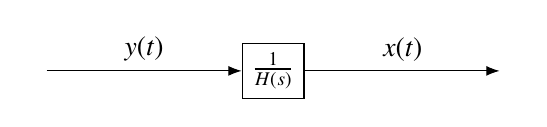
\begin{tikzpicture}[auto, node distance=4cm,>={Latex}]
  % Define blocks
  \node (input) at (0,0) {};
  \node [draw, rectangle] (H) at (3,0) {$\frac{1}{H(s)}$}; 
  \node (output) at (6,0) {};

  % Connect blocks with right arrows
  \draw [->] (input) -- node[midway, above] {$y(t)$} (H);
  \draw [->] (H) -- node[midway, above] {$x(t)$} (output);
\end{tikzpicture}


\textbf{Solution:}
\fi
\begin{table}[!ht]
\renewcommand\thetable{1}
   \centering
\begin{tabular}{|c|c|c|}
  \hline
  \textbf{Symbol} & \textbf{Value} & \textbf{Description}\\
  \hline
  $L$ &  $10mH$ & Inductance\\
  \hline 
  $C$ &  $100mu F$ & Capacitance \\
  \hline
  $R_1$ &  $2\ohm$ & Resistance\\
  \hline
  $R_2$ & $2\ohm$ & Resistance\\
  \hline
    $R_3$ & $3\ohm$ & Resistance\\
  \hline
  $V_L$ & $??$ & Voltage across the inductor\\
  \hline
    $V_C$ & $??$ & Voltage across the capacitor\\
  \hline
  $I_0$ & $10 A$ & DC current source\\
  \hline
  $I_L$ & $??$ & Current in inductor\\
    \hline
\end{tabular}
\caption{Input Parameter}
\end{table}


At t=$0^-$, inductor behaves as wire and capacitor as open switch,

\begin{circuitikz}
    \draw (0,0) to [R, R=$3\ohm$] (0,3);
   \draw (0,3)-- (0,4);
   \draw (0,4) -- (3,4);
   \draw (2.5,0) to [american current source, l=$10\text{A,}\text{DC}$] (2.5,4);
    \draw (3,4) to (3,5);
    \draw (3,5) to[R, l=$2\ohm$,i=$I_L(0^-)$] (8,5);
    \draw (3,4)to (3,3)to (4,3) to[R, l=$2\ohm$] (5,3);
    \draw (5,3)to (6,3) ;
    % Draw open circuit
    \draw (7,3) to [open, v=$+\quad V_C(0^-)\quad-$] (6,3);
     \draw (7,3) to(8,3);
    \draw (8,5) --(8,3);
    \draw (8,4) -- (9,4);
    \draw (9,4)-- (9,0);
    \draw(9,0)--(0,0);
\end{circuitikz}\\

after current distribution
\begin{equation}
    I_L(0^-) = 10A\brak{\frac{3}{3+2}}=6 A\\
    \label{eq:23.29.1}
 \end{equation}  
 \begin{equation}
    V_C(0^-)= 6\times2= 12 V
     \label{eq:23.29.2}
\end{equation}

For $t>0$, the switch is opened.

\begin{circuitikz}[american]
   \draw (0,0) to [current source,
   l=$\frac{10}{s}$] (0,4);
    \draw (0,4)-- (1,4) to(1,5)to[R, l=$2\ohm$, i=$I_L$] (4,5);
    \draw  (4,5) to[L, l=$10mH$,]  (6,5);
    \draw  (8,5) to[sV, V=$LI_L(0^-)$] (6,5);
    \draw (1,4)to (1,2)to[R, l=$2\ohm$, i=$\brak{\frac{10}{s}-I_L}$] (4,2);
    \draw (4,2) to [C, l=$100\mu F$,] (6,2);
    \draw  (6,2) to[sV, V=$\frac{V_C(0^-)}{s}$] (8,2);
    \draw (8,5) --(8,2);
    \draw (8,4) -- (9,4);
    \draw (9,4)-- (9,0);
    \draw(9,0)-- (0,0);
\end{circuitikz}

Using KVL,\\
\begin{multline}
2I_L+LsI_L-LI_L(0^-)-\frac{V_C(0^-)}{s}-\frac{1}{Cs}\brak{\frac{10}{s}-I_L}-2\brak{\frac{10}{s}-I_L}=0
   \label{eq:23.29.3}
\end{multline}
From \eqref{eq:23.29.1}, \eqref{eq:23.29.2}, \eqref{eq:23.29.3}
\begin{align}
I_L=\frac{6s^2+3200s+10^7}{s\brak{s^2+400s+10^6}}
\label{eq:23.29.4}\\
V_L(s)=I_L(sL)
\end{align}

Using \eqref{eq:23.29.4}
\begin{align}
V_L(s)=\frac{0.06s^2+32s+10^5}{\brak{s^2+400s+10^6}}
\label{eq:23.29.6}
\end{align}

Some Result:
\begin{align}
\frac{1}{s^2+400s+10^6} &\system{L} \brak{e^{-200t}}\frac{\sin(400\sqrt{6}t)}{400\sqrt{6}}
   \label{eq:23.29.7}\\
\frac{s}{s^2+400s+10^6} &\system{L} \brak{e^{-200t}}\frac{\brak{2\sqrt{6}\cos(400\sqrt{6}t)-\sin(400\sqrt{6}t)}}{2\sqrt{6}}
   \label{eq:23.29.8}\\
\frac{s^2}{s^2+400s+10^6} &\system{L} \brak{-e^{-200t}}\frac{\brak{2300\sin(400\sqrt{6}t)+400\sqrt{6}\cos(400\sqrt{6}t)}}{\sqrt{6}}
   \label{eq:23.29.9}
\end{align}

Inverse Laplace transform of \eqref{eq:23.29.6} Using \eqref{eq:23.29.7},\eqref{eq:23.29.8}, \eqref{eq:23.29.9}

\begin{multline}
	V_L(t)=e^{-200t}\brak{-0.06\brak{\frac{\brak{2300\sin(400\sqrt{6}t)+400\sqrt{6}\cos(400\sqrt{6}t)}}{\sqrt{6}}}+32\brak{\frac{\brak{2\sqrt{6}\cos(400\sqrt{6}t)-\sin(400\sqrt{6}t)}}{2\sqrt{6}}}}\\+e^{-200t}\brak{10^5\frac{\sin(400\sqrt{6}t)}{400\sqrt{6}}}
\end{multline}
at t=$0^+$
\begin{align}
    V_L(0^+)= -24+32=8V
\end{align}
Hence at t=$0^+$ voltage across inductor is 8V
\begin{figure}[!h]
    \centering
    \includegraphics[width = \columnwidth]{2023/EE/29/figs/c.png}
    \caption{plot of voltage as function of t}
\end{figure}
%\end{document}
